\section{Experiments}
We empirically validate our theoretical framework and illustrate the distinct behaviors of the reject-option predictors through a synthetic experiment.

\paragraph{Data} We employ a setup similar to the running example, but to increase model complexity, we use a third-degree polynomial instead of a linear regression model. For each trial, we define a ground-truth data-generating function by sampling a parameter vector $\#\theta$ from a zero-mean Gaussian prior. This vector, $\#\theta$, represents the coefficients of the cubic polynomial. The prior covariance is a diagonal matrix with a variance of $1$ for the intercept term and $0.1$ for all other coefficients. We then generate a training set $D$ of size $m$ by drawing i.i.d. samples $x \sim \mathcal{N}(0, 1)$ and generating corresponding labels $y$ from the true function with added heteroscedastic noise. Specifically, the labels are sampled according to the following distribution: $p(y|x, \#\theta) = \mathcal{N}( y\mid f(x; \#\theta), v(x))$, where $f(x; \#\theta)$ is the true polynomial function and the variance $v(x) = 0.1 + 0.04(x + 8)^2$.

%We employ similar setup as in the running example, but insteat of linear regression model we use polynomial of degree 3 to increase model complexity. For each trial, we first define a ground-truth data-generating function by sampling a parameter vector $\#\theta^*$ from a zero-mean Gaussian prior, where $\#\theta^*$ represents the coefficients of a cubic polynomial. The prior covariance is a diagonal matrix with a variance of $1$ for the intercept term and $0.1$ for all other coefficients. We then generate a training set $D$ of size $m$ by drawing i.i.d. samples $x \sim \mathcal{N}(0, 1)$ and generating corresponding labels $y$ from the true function with added heteroscedastic noise. Specifically, $p(y|x,\#\theta) = \SN( y\mid f(x; \#\theta^*), v(x))$, where $v(x) = 0.1 + 0.04 \cdot (x + 8)^2$ is the variance.

\paragraph{Compared predictors} We compare three reject-option strategies:
i) the Bayesian reject-option predictor \equ{equ:TotalRejectBL}, ii)
the proposed epistemic reject-option predictor~\equ{equ:OptEpistRejOptPred}, and a plug-in reject-option predictor using $\hat{h}(x) = h(x, \hat{\theta})$ and $\hat{r}(x) = r(x, \hat{\theta})$, where $\hat{\theta}$ is the maximum-likelihood estimate.
As previously shown, the inference for the Bayesian and the epistemic predictors has an analytical solution.



%} (Figure \ref{fig:BayesianRejectOpt}), the proposed \textit{epistemic reject-option predictor} (Figure \ref{fig:EpistemicRejectOpt}), and the \textit{plug-in aleatoric predictor}, which first learns a predictor $\hat{h}(x)$ via maximum-likelihood estimation of $\#\theta$, and then abstains based on the known aleatoric uncertainty $r^*(x)=v(x)$.
% We then perform Bayesian inference to compute the posterior distribution over the model parameters $p(\#\theta\mid D)$. We compare three reject-option strategies: The \textit{Bayesian reject-option predictor} (Figure \ref{fig:BayesianRejectOpt}), the proposed \textit{epistemic reject-option predictor} (Figure \ref{fig:EpistemicRejectOpt}), and the \textit{plug-in aleatoric predictor}, which first learns a predictor $\hat{h}(x)$ via maximum-likelihood estimation of $\#\theta$, and then abstains based on the known aleatoric uncertainty $r^*(x)=v(x)$.

\paragraph{Evaluation metric} Following the standard approach in the reject-option literature, we evaluate performance using the Regret–Coverage curve, which plots the expected regret on non-rejected inputs against the coverage (i.e., the proportion of accepted inputs) across all possible rejection thresholds $\epsilon$ or $\delta$. Performance is summarized by the Area under the Regret–Coverage curve (AuReC), where a lower value indicates better performance. 
%The AuReC corresponds to the expected regret on non-rejected inputs when the rejection cost is drawn uniformly at random. 
Experiments are repeated for various training set sizes $m$, and results are averaged over 3000 independent trials.

% For each learned predictor, we generate a \textit{Regret-Coverage} curve by plotting the expected regret against the coverage for all possible rejection thresholds $\epsilon$ or $\delta$. 
%Performance of the predictor is summarized by the \textit{Area under the Regret-Coverage} (AuReC) curve, where a lower area indicates better performance. The experiment is repeated with various training data sizes $m$ and the results are averaged over 3000 trials.

\paragraph{Results}
The performance curves in Figure \ref{fig:synthetic_experiment} confirm our claims. Our proposed epistemic predictor is the top performer for regret minimization, consistently achieving the lowest AuReC across all dataset sizes $m$. The results also highlight how different types of uncertainty affect performance at different data scales. With small datasets, epistemic uncertainty is high and dominates the total uncertainty. In this regime, the performance of the Bayesian and epistemic predictors is nearly identical. As the dataset grows, epistemic uncertainty diminishes, and the total uncertainty becomes dominated by the aleatoric component. As expected, this causes the Bayesian predictor's performance to converge with that of an aleatoric-only predictor.

%The final performance curves shown in Figure \ref{fig:synthetic_experiment} empirically validate our claims. 
%For regret minimization, the proposed epistemic reject-option predictor achieves the lowest AuReC across all data sizes. 
%We also observe that for small $m$, where epistemic uncertainty is high and dominates the total uncertainty, the performance of the Bayesian and epistemic predictors is nearly identical. 
%Conversely, as $m$ becomes large, epistemic uncertainty vanishes, and the total uncertainty becomes dominated by the aleatoric component. 
%Consequently, the performance of the Bayesian predictor converges towards that of the aleatoric-only predictor as expected.

\begin{figure}[htb]
    \centering
    \begin{minipage}[l]{\linewidth}
        \centering
        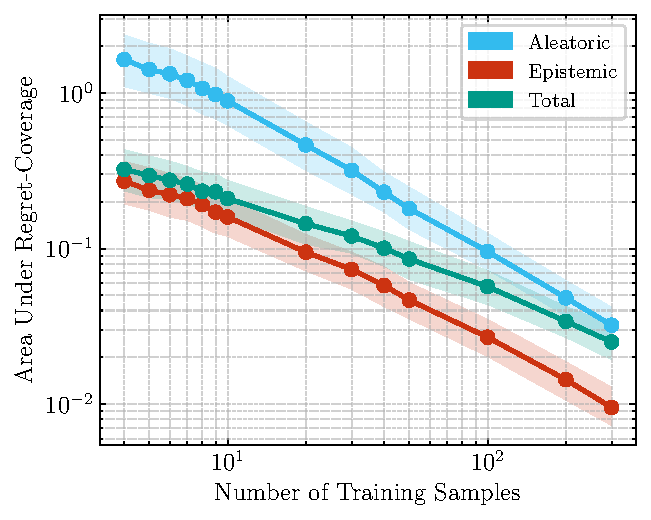
\includegraphics[width=\linewidth]{figures/synthetic_experiment.pdf}
        \captionof{figure}{
        %Performance of different reject-option predictors on a synthetic polynomial regression task. The plot shows the Area under the Regret-Coverage (AuReC) curve versus the number of training samples. Lower AuReC indicates better performance. The predictor using epistemic uncertainty consistently outperforms those using total or aleatoric uncertainty for regret minimization. Shaded regions show the central 20\% interval of results across 3000 trials.
        The performance of different reject-option predictors in a synthetic polynomial regression task. The plot shows the Area under the Regret-Coverage (AuReC) curve, where a lower value indicates superior performance, plotted against the number of training samples. The results demonstrate that the proposed predictor using epistemic uncertainty consistently achieves lower regret and outperforms predictors that rely on total or aleatoric uncertainty. Shaded areas indicate the central $20\%$ interval of outcomes across 3000 independent trials.        
        }
        \label{fig:synthetic_experiment}
    \end{minipage}
\end{figure}
